% Asset ID: AS1AlgebraicMethodsProofTikZ-005
% Source: Chapter 7b Algebraic Methods, Proof transcript
% Related lesson section: Worked Example 8; Core Theory
% Purpose: Proof by exhaustion using 3n, 3n+1, 3n-1 for cube numbers.

\documentclass[tikz,border=8pt]{standalone}
\usepackage{amsmath}
\usetikzlibrary{arrows.meta,positioning}
\begin{document}
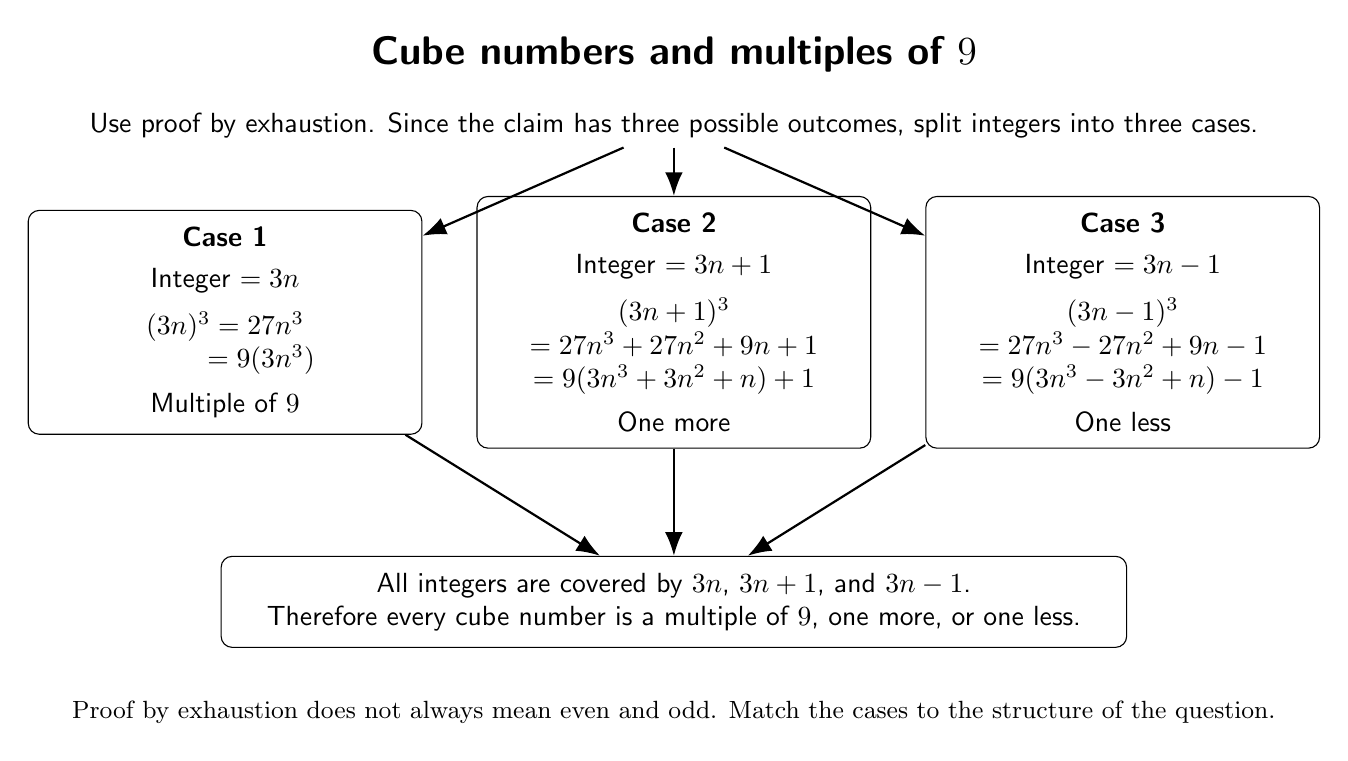
\begin{tikzpicture}[font=\sffamily,casebox/.style={draw,rounded corners,align=center,minimum width=5.0cm,minimum height=2.4cm,inner sep=6pt},conclusion/.style={draw,rounded corners,align=center,minimum width=11.5cm,minimum height=1.15cm,inner sep=6pt},arr/.style={-{Latex[length=3mm]}, thick}]
\node[font=\sffamily\bfseries\Large, align=center] at (0,4.75){Cube numbers and multiples of \(9\)};
\node[align=center] (start) at (0,3.85){Use proof by exhaustion. Since the claim has three possible outcomes, split integers into three cases.};
\node[casebox] (caseone) at (-5.7,1.35){\textbf{Case 1}\\[3pt]Integer \(=3n\)\\[5pt]\((3n)^3=27n^3\)\\\(\phantom{(3n)^3}=9(3n^3)\)\\[4pt]Multiple of \(9\)};
\node[casebox] (casetwo) at (0,1.35){\textbf{Case 2}\\[3pt]Integer \(=3n+1\)\\[5pt]\((3n+1)^3\)\\\(=27n^3+27n^2+9n+1\)\\\(=9(3n^3+3n^2+n)+1\)\\[4pt]One more};
\node[casebox] (casethree) at (5.7,1.35){\textbf{Case 3}\\[3pt]Integer \(=3n-1\)\\[5pt]\((3n-1)^3\)\\\(=27n^3-27n^2+9n-1\)\\\(=9(3n^3-3n^2+n)-1\)\\[4pt]One less};
\node[conclusion] (done) at (0,-2.2){All integers are covered by \(3n\), \(3n+1\), and \(3n-1\).\\Therefore every cube number is a multiple of \(9\), one more, or one less.};
\draw[arr] (start) -- (caseone);\draw[arr] (start) -- (casetwo);\draw[arr] (start) -- (casethree);\draw[arr] (caseone) -- (done);\draw[arr] (casetwo) -- (done);\draw[arr] (casethree) -- (done);
\node[align=center, font=\small] at (0,-3.6){Proof by exhaustion does not always mean even and odd. Match the cases to the structure of the question.};
\end{tikzpicture}
\end{document}
